\documentclass[a4paper, twoside]{article}
\usepackage[utf8]{inputenc} % Especifica la codificación de caracteres de los documentos.
\usepackage[spanish]{babel} % Indica que el documento se escribirá en español.
\usepackage[top=3cm, bottom=2.5cm, inner=1.5cm, outer=2.5cm]{geometry} % Márgenes personalizados
\usepackage{subfiles} % Paquete para incluir el preambulo en los sub archivos.
\usepackage{afterpage} % Permite añadir páginas despues de una página dada.
\usepackage{hyperref} % Permite incluir enlaces en los archivos.
\usepackage{lastpage} % Paquete para poder contabilizar el total de páginas del documento.
\usepackage{fancyhdr} % Permite personalizar los header y footer del documento.
\usepackage{graphicx} % Permite incluir gráficos
\usepackage[hang, bf]{caption} % Personaliza los subtítulos de las figuras y tablas
\usepackage{float} % Permite posicionar mejor las figuras y tablas
\usepackage{amsmath} % Comandos para la escritura de fórmulas matemáticas de mayor complejidad
\usepackage{amsfonts} % Proporciona fuentes matemáticas
\usepackage{amssymb} % Proporciona símbolos matemáticos de la American Mathematical Society
\usepackage{cancel}

% Defino la ruta de los paquetes personalizados para el apunte
\newcommand{\rutapaquetes}{./paquetes-apunte}

\usepackage[mostrarlicencia]{\rutapaquetes/caratula} % Caratula personalizada (cargada desde caratula.sty)
\usepackage[ocultarrevisores]{\rutapaquetes/colaboradores} % Seccion de colaboradores (cargada y creada con colaboradores.sty)
\usepackage{\rutapaquetes/historial} % Seccion de historial de cambios (cargada y creada con historial.sty)

% Define los estilos de los enlaces interpretados por el paquete hyperref
\hypersetup{
	colorlinks=true,   % false: boxed links; true: colored links
	linkcolor=black,   % color of internal links (change box color with linkbordercolor)
	citecolor=green,   % color of links to bibliography
	filecolor=magenta, % color of file links
	urlcolor=blue,     % color of external links
}

\newcommand{\imgdir}{../resources/images} % Ruta de las imágenes

% Define los directorios de las imágenes y gráficos
\graphicspath{ {\imgdir/} {\rutapaquetes/} }

% Defino el comando "\nombremateria" para no harcodear el nombre en varios lugares.
\newcommand{\nombremateria}{Matemática Discreta (61.07 - 81.11)}

% Define el pagestyle personalizado
\pagestyle{fancy}
\fancyhf{}
\renewcommand{\sectionmark}[1]{\markboth{}{\thesection\ \ #1}}
% Define header para pagina par
\fancyhead[ER]{\rightmark}
% Define header para pagina impar
\fancyhead[OL]{\rightmark}
% Define footer para pagina par
\fancyfoot[EL]{\nombremateria \hspace{0.1cm} - Resumen} % Nombre del apunte a la izquierda
\fancyfoot[ER]{Página \thepage\ de \pageref{LastPage}} % Numero de pagina a la derecha
% Define footer para pagina impar
\fancyfoot[OL]{Página \thepage\ de \pageref{LastPage}} % Numero de pagina a la izquierda
\fancyfoot[OR]{\nombremateria \hspace{0.1cm} - Resumen} % Nombre del apunte a la derecha

\renewcommand{\footrulewidth}{0.4pt} % Agrego linea que separa el footer

% Configura la caratula
\materia{\nombremateria}
\tipoapunte{Resumen}
%\tema{Tema de la Materia}
%\subtema{Subtema}

\makeatletter
\newcommand{\rmnum}[1]{\romannumeral #1}
\newcommand{\Rmnum}[1]{\expandafter\@slowromancap\romannumeral #1@}
\makeatother

\begin{document}

\maketitle

\tableofcontents

\subfile{\rutapaquetes/sobre-el-proyecto.tex} % Incluye información sobre el proyecto FIUBA Apuntes

\section{Lógica Proposicional}
Una proposición es un enunciado del lenguaje al que tiene sentido asignarle un valor de verdad o falsedad.

\subsection{Conectores lógicos}
\begin{enumerate}
	\item \textbf{Negación}: Es un operador que se ejecuta, sobre un único valor de verdad, devolviendo el valor contradictorio de la proposición considerada.
		\begin{center}
			\begin{tabular}{|c|c|}
			\hline
			\textbf{p} & $\lnot$ \textbf{p} \\
			\cline{0 - 1}
			\hline
			0 & 1 \\
			1 & 0 \\
			\hline
			\end{tabular}
		\end{center}
	
	\item \textbf{Conjunción}: Es un operador que devuelve verdadero cuando ambas proposiciones son verdaderas, y falso en cualquier otro caso.
		\begin{center}
			\begin{tabular}{|c|c|c|}
			\hline
			\textbf{p} & \textbf{q} & \textbf{p} $\wedge$ \textbf{q}\\
			\cline{0 - 1}
			\hline
			0 & 0  & 0\\
			0 & 1  & 0\\
			1 & 0  & 0\\
			1 & 1  & 1\\
			\hline
			\end{tabular}
		\end{center}
	
	\item \textbf{Disyunción}: Es un operador que devuelve verdadero cuando una de las proposiciones es verdadera, o cuando ambas lo son, y falso cuando ambas son falsas.
		\begin{center}
			\begin{tabular}{|c|c|c|}
			\hline
			\textbf{p} & \textbf{q} & \textbf{p} $\lor$ \textbf{q}\\
			\cline{0 - 1}
			\hline
			0 & 0  & 0\\
			0 & 1  & 1\\
			1 & 0  & 1\\
			1 & 1  & 1\\
			\hline
			\end{tabular}
		\end{center}
	
	\item \textbf{Disyunción excluyente}: Es un operador que devuelve verdadero cuando una de las proposiciones es verdadera, y falso cuando ambas son verdaderas o falsas.
		\begin{center}
			\begin{tabular}{|c|c|c|}
			\hline
			\textbf{p} & \textbf{q} & \textbf{p} $\veebar$ \textbf{q}\\
			\cline{0 - 1}
			\hline
			0 & 0  & 0\\
			0 & 1  & 1\\
			1 & 0  & 1\\
			1 & 1  & 0\\
			\hline
			\end{tabular}
		\end{center}
	
	\item \textbf{Implicación} \footnote{No cumple propiedad conmutativa $p \to q \neq q \to p$}: Es un operador que devuelve falso sólo cuando la primera proposición es verdadera y la segunda falsa, y verdadero en cualquier otro caso.
		\begin{center}
			\begin{tabular}{|c|c|c|}
			\hline
			\textbf{p} & \textbf{q} & \textbf{p} $\to$ \textbf{q}\\
			\cline{0 - 1}
			\hline
			0 & 0  & 1\\
			0 & 1  & 1\\
			1 & 0  & 0\\
			1 & 1  & 1\\
			\hline
			\end{tabular}
		\end{center}
	
	\item Implicación contrarecíproca $\equiv$ Implicación
		\begin{center}
			\begin{tabular}{|c|c|c|}
			\hline
			\textbf{p} & \textbf{q} & \textbf{p} $\leftarrow$ \textbf{q}\\
			\cline{0 - 1}
			\hline
			0 & 0  & 1\\
			0 & 1  & 0\\
			1 & 0  & 1\\
			1 & 1  & 1\\
			\hline
			\end{tabular}
		\end{center}
	
	\item \textbf{Doble Implicación}: Es un operador que devuelve verdadero cuando ambas proposiciones tienen el mismo valor de verdad, y falso cuando sus valores de verdad difieren.
		\begin{center}
			\begin{tabular}{|c|c|c|}
			\hline
			\textbf{p} & \textbf{q} & \textbf{p} $\leftrightarrow$ \textbf{q}\\
			\cline{0 - 1}
			\hline
			0 & 0  & 1\\
			0 & 1  & 0\\
			1 & 0  & 0\\
			1 & 1  & 1\\
			\hline
			\end{tabular}
		\end{center}
\end{enumerate}

\subsection{Tipos de proposiciones}
\begin{itemize}
	\item \emph {Tautología:} Esquema proposicional que toma un valor \textbf{verdadero}, independientemente de las proposiciones que la integran. 

	\item \emph {Contradicción:} Esquema proposicional que toma un valor \textbf{falso}, independientemente de las proposiciones que la integran. 

	\item \emph {Contingencia:} Esquema proposicional que puede resultar \textbf{verdadero o falso}.
\end{itemize}

\subsection{Leyes de la lógica}

\begin{enumerate}
	\item Conmutatividad de $\wedge$ y $\lor$
		\begin{center}
			$ p \wedge q \equiv q \wedge p \quad$ y $\quad p \lor q \equiv q \lor p $
		\end{center}

	\item Asociatividad de $\wedge$ y $\lor$
		\begin{center}
			$ (p \wedge q) \wedge r \equiv p \wedge (q \wedge r) \quad$ y $\quad (p \lor q) \lor r \equiv p \lor (q \lor r) $
		\end{center}

	\item Doble distributividad
		\begin{center}
			$ p \lor (q \wedge r) \equiv (p \lor q) \wedge (p \lor r) \quad$ y $\quad p \wedge (q \lor r) \equiv (p \wedge q) \lor (p \lor r)$ 
		\end{center}

	\item Identidad
		\begin{center}
			$ p \lor 1 \equiv 1 $\\
			$ p \lor 0 \equiv p $\\
			$ p \wedge 1 \equiv p $\\
			$ p \wedge 0 \equiv 0 $
		\end{center}

	\item Idempotencia
		\begin{center}
			$ (p \lor p) \equiv p  \quad$ y $\quad (p \wedge p) \equiv p $
		\end{center}

	\item Doble negación
		\begin{center}
			$ \lnot (\lnot p) \equiv p $
		\end{center}

	\item Absorción
		\begin{center}
			$ (p \wedge q) \lor p \equiv p \quad$ y $\quad (p \lor q) \wedge p \equiv p $
		\end{center}

	\item Leyes de De Morgan
		\begin{center}
			$ \lnot (p \lor q) \equiv (\lnot p  \wedge \lnot q) \quad$ y $\quad \lnot (p \wedge q) \equiv (\lnot p  \lor \lnot q) $
		\end{center}
\end{enumerate}

\subsection{Métodos para demostrar una implicación $p \to q$}
\subsubsection{Método Directo}
Suponer $v(p) = 1$ y llegar a que $v(q) = 1$.

\subsubsection{Método indirecto o del contrarecíproco}
Demostrar la verdad de la implicación \emph{contrarecíproca} por método directo

Suponer $v(\lnot p) = 1$ y llegar a que $v(\lnot q) = 1$.\\

\textbf{Ejemplo:} Quiero demostrar $p \to q \equiv$ ab es par $\to$ (a es par $\lor$ b es par).
Entonces, demuestro $v(q) = 0$ , esto se logra demostrando los 3 casos donde $v(p) = 0$.

\begin{center}
	$v(q)=0\left\{ \begin{array}{c}
	v(a)=0\wedge v(b)=0\\
	v(a)=1\wedge v(b)=0\\
	v(a)=0\wedge v(b)=1\end{array}\right.$
\end{center}

\subsubsection{Método del Absurdo o Contradicción}
Supongo $\left\{ \begin{array}{c} v(p)=1\\ v(q)=0\end{array}\right.$ e intento llegar a un absurdo.

\newpage
\section{Lógica de Predicados}
\subsection{Función Proposional}
No son proposiciones debido a que \textbf{no} se le puede asignar un valor de verdad, ya que depende de una variable.\\

Ej: $P(x) = x$ es inteligente.\\

Una vez especializada la variable, se transforma en una proposición.

\subsection{Cuantificación de una variable}
\begin{itemize}
	\item Universal $\forall x \in D: P(x)$
		\begin{itemize}
			\item \emph{Verdadero}: Hay que mostrar que todos los elementos de D tienen la propiedad P.
			\item \emph{Falso}: Basta mostrar un elemento de D que \textbf{no} tenga la propiedad P.
		\end{itemize}
	
	\item Existencial $\exists x \in D: P(x)$
		\begin{itemize}
			\item \emph{Verdadero}: Basta mostrar un elemento de D que tenga la propiedad P.
			\item \emph{Falso}: Hay que mostrar que todos los elementos de D \textbf{no} tienen la propiedad P.
		\end{itemize}
\end{itemize}

\subsubsection{Propiedades}
\begin{itemize}
	\item $\forall y: \exists x \neq \exists x: \forall y$
	\item $\forall x: \forall y \equiv \forall y: \forall x$
	\item $\exists x: \exists y \equiv \exists y: \exists x$
	\item $\neg\left[\forall x \in D: P(x)\right] \equiv \exists x \in D: \neg P(x)$
	\item $\neg\left[\exists x \in D: P(x)\right] \equiv \forall x \in D: \neg P(x)$
\end{itemize}

\newpage
\section{Conjuntos}
	\subsection{Álgebra de conjuntos}
	\begin{itemize}
		\item \emph{Igualdad}: $ A = B \leftrightarrow (A \subseteq B \wedge B \subseteq A)$	
		\item \emph{Inclusión}: $A \subseteq B \leftrightarrow (\forall x \in U):(x \in A \rightarrow x \in B)$	
		\item \emph{Union}: La unión de dos conjuntos $A$ y $B$ es el conjunto $A \cup B$ que contiene cada elemento que está por lo menos en uno de ellos.

		\item \emph{Intersección}: La intersección de dos conjuntos $A$ y $B$ es el conjunto $A \cap B$ que contiene todos los elementos comunes de $A$ y $B$.

		\item \emph{Diferencia}:  La diferencia entre dos conjuntos $A$ y $B$ es el conjunto $A \setminus B$ que contiene todos los elementos de $A$ que no pertenecen a $B$.

		\item \emph{Complemento}: El complemento de un conjunto $A$ es el conjunto $A^\complement$ que contiene todos los elementos (respecto de algún conjunto referencial) que no pertenecen a $A$.

		\item \emph{Diferencia simétrica}: La diferencia simétrica de dos conjuntos $A$ y $B$ es el conjunto $A \Delta B$ con todos los elementos que pertenecen, o bien a $A$, o bien a $B$, pero no a ambos a la vez.
	\end{itemize}
	
	\begin{figure}
		\centering
		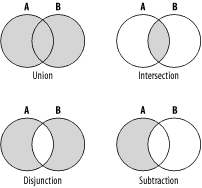
\includegraphics{set}
		\caption{Diagramas de Venn}
		\label{fig:set}
	\end{figure}
	
	\subsection{Relaciones de conjuntos}
	Sea $A$ un conjunto. Se llama \emph{Relación en el conjunto} $A$ a todo conjunto $R:R \subseteq A \times A$
	
	\vspace{0.25cm}
	Definiciones:
	\begin{enumerate}

		\item Producto cartesiano: $\times$
		
		$A \times B = \{(a,b) a \in A \wedge b \in B\}$
		
		\item Cardinal de $A$: $|A| = $ Cantidad de elementos de $A$ 
		
		\item Conjunto de partes : $ P\left[A\right] = \left\{  \Rmnum{10}: \Rmnum{10} \subseteq A \right\}$
		
		$ P\left[\left\{ 1,2,3 \right\}\right] = \left\{ \varnothing , \left\{1\right\}, \left\{2\right\} , \left\{3\right\} , \left\{1,2\right\} , \left\{2,3\right\} , \left\{1,3\right\}, \left\{1,2,3\right\} \right\}$
		
		$|A| = n \rightarrow |P\left[A\right]| = 2^n$
		
		\item Compresión $\left\{ \left\{ x,y \right\} \in A \times A: x+y \leq \alpha \right\}$
		
	\end{enumerate}	
	
	Relaciones:
	\begin{itemize}
		\item Complementaria: $\overline{R} = \left\{ \left\{ (x,y) \right\} \in A \times A: (x,y) \notin R\right\}$
		
		\item Inversa: $R^{-1} = \left\{ \left\{ (x,y) \right\} \in A \times A: (y,x) \in R\right\}$
		
		\item  Unión: $R \subseteq A \times A \wedge S \subseteq A \times A$
		
		\begin{center}
		$R \cup S = \left\{ \left\{ (x,y) \right\} \in A \times A: (x,y) \in R \lor (x,y) \in S \right\}$
		\end{center}		

		\item Intersección: $R \subseteq A \times A \wedge S \subseteq A \times A$
		
		\begin{center}
		$R \cup S = \left\{ \left\{ (x,y) \right\} \in A \times A: (x,y) \in R \wedge (x,y) \in S \right\}$
		\end{center}
		
		\item Reflexiva: $\forall x \in A: (x,x) \in R$
						 $\forall x \in A: x \mathcal{R} x$
		
		\item Simétrica: $\forall x,y \in A: (x,y) \in R \rightarrow (y,x) \in R$
				
		\item Antisimétrica: $\forall x,y \in A: (x,y) \in R \wedge (y,x) \in R \rightarrow x = y$
		
		\item Transitiva: $\forall x,y,z \in A: (x,y) \in R \wedge (y,z) \in R \rightarrow (x,z) \in R$
		
		\item Equivalencia: $\left\{ \begin{array}{c}
							\text{Reflexiva}\\
							\text{Transitiva}\\
							\text{Simétrica}\end{array}\right.$
		
		\item Orden: $\left\{ \begin{array}{c}
							\text{Reflexiva}\\
							\text{Antisimétrica}\\
							\text{Transitiva}\end{array}\right.$
	\end{itemize}
	
	Ejemplo:
	
	$A = \left\{1,2,3\right\}$
	
	$R_1 = \left\{ \left\{ 1,2\right\} , \left\{ 2,1\right\}  , \left\{ 1,3\right\}  , \left\{ 3,1\right\}  \right\}$

	\subsection{Representación matricial}
	Una relación tiene asociada una \emph{matriz de relación} la cual 
	contiene toda la informacion sobre la misma.
	
	Ejemplo:
	
	$A = \left\{1,2,3,4\right\}$
	
	$R = \left\{ \left\{ 1,1\right\} , \left\{ 1,2\right\}  , \left\{ 1,4\right\}  , \left\{ 2,1\right\} , \left\{ 2,3\right\} , \left\{ 3,2\right\} , \left\{ 4,1\right\} , \left\{ 4,4\right\} \right\}$

	$M_R =$ Matriz de la relación $R$ 
	
	$ M_R \left[\begin{array}{cccc}
	1 & 1 & 0 & 1\\
	1 & 0 & 1 & 0\\
	0 & 1 & 0 & 0\\
	1 & 0 & 0 & 1\end{array}\right]$
	
	$R_1$ es simétrica, no reflexiva y no transitiva.
	
	¿Cómo puedo obtener esta información observando la matriz?
	
	\begin{itemize}
		\item{Reflexión}  $I \leq M_R$
		\item{Simetría} $M_R = {M_R}^T$
		\item{Antisimetría} $M_R \cap {M_R}^T \leq I$
		\item{Transitividad} ${M_R}^2 = M_R M_R \leq M_R$
	\end{itemize}
	
	Se considera que una matriz (de tamaño $m \times n$) es mayor o igual que otra (del mismo tamaño) si:
	\begin{center}
	$c_{i,j} \leq d_{i,j} \quad \forall i,j$ tal que $\quad 1 \leq i \leq m \quad , \quad  1 \leq j \leq n $
	\end{center}	

	\subsection{Clases de equivalencia}
	
	Sea $\mathcal{R}$ una relación de equivalencia en $A$ , $\forall a \in A $ se define:
	$\overline{a} = \left[a\right] = cl(a) = \left\{x \in A: x\mathcal{R} a\right\}$
	
	Teorema: Sea R una relación de equivalencia en $A$, se verifica:
	\begin{enumerate}
		\item $\forall a \in A: \left[a\right] \subseteq A$
		
		\item $\forall a \in A: \left[a\right] \neq \varnothing$
		
		\item $\forall a,b \in A: a\mathcal{R} b \leftrightarrow \left[a\right] = \left[b\right]$
		
		\item $\forall a,b \in A: a \cancel{\mathcal{R}} b \leftrightarrow \left[a\right] \cap \left[b\right]= \varnothing$
	\end{enumerate}
	
	\subsection{Partición}
	Una partición de un conjunto A es la familia de subconjuntos $\left\{ A_i: 1 \leq i \leq n\right\}$ que cumple las siguientes condiciones:
	\begin{enumerate}
		\item $A_i \subseteq A \forall i: 1 \leq i \leq n$
		
		\item $A_i \neq \varnothing \quad \forall i: 1 \leq i \leq n$
		
		\item $\bigcup_{i\in I} A_i = A$
		
		\item $A_i \cap A_j \neq \emptyset \quad \forall i,j: 1\leq i ; \quad j \leq n	\quad \wedge (i \neq j)$
	\end{enumerate}
	
	\emph{El conjunto de las clases de equivalencia de $A$ forma una partición de $A$}
	
	\subsection{Relación de orden}
	Sea $A$ un conjunto dado no vacío y $\mathcal{R}$ una relación binaria definida en $A$ , entonces decimos que $\mathcal{R}$  es una relación de orden \emph{parcial} si cumple las siguientes propiedades:
	\begin{itemize}
		\item Reflexiva
		\item Antisimétrica
		\item Transitiva
	\end{itemize}
	
	Si $(A,\mathcal{R})$ es un conjunto parcialmente ordenado, decimos que $A$ es \emph{totalmente ordenado} si $\forall x,y \in A$ ocurre que $x\mathcal{R}y$ o $y\mathcal{R}x$.
	Si esto ocurre decimos que $\mathcal{R}$ es un \emph{orden total}.
	
        \begin{description}
            \item[Elemento maximal] Si $A$ es un conjunto parcialmente ordenado, entonces un elemento  $x \in A$ es 
            un elemento \emph{maximal} de $A$ si para todo $a \in A, a \neq x \rightarrow x \cancel{\mathcal{R}} a$.
            \item[Elemento minimal] Si $A$ es un conjunto parcialmente ordenado, entonces un elemento  $y \in A$ es 
            un elemento \emph{minimal} de $A$ si para todo $b \in A, b \neq y \rightarrow b \cancel{\mathcal{R}} y$.
            \item[Maximo] Si $A$ es un conjunto parcialmente ordenado, entonces un elemento  $x \in A$ es 
            un elemento \emph{máximo} de $A$ si para todo $a \in A,a \mathcal{R} x$.
            \item[Mínimo] Si $A$ es un conjunto parcialmente ordenado, entonces un elemento  $y \in A$ es 
            un elemento \emph{mínimo} de $A$ si para todo $b \in A,y \mathcal{R} b$.
        \end{description}
            Sea $(A,\mathcal{R})$ un conjunto parcialmente ordenado con $B \subseteq A$.

        \begin{description}  
            \item[Cota superior]  Un elemento  $x \in A$ es una \emph{cota superior} de $B$ si para todo $b \in B,b \mathcal{R} x$.
            \item[Cota inferior]  Un elemento  $y \in A$ es una \emph{cota inferior} de $B$ si para todo $b \in B,y \mathcal{R} b$.
            \item[Supremo] Un elemento $x' \in A$ es \emph{supremo} de $B$, si es una cota superior de $B$ y $x'\mathcal{R}x''$ 
            para todas las demás cotas superiores $x'' \in B$. \textbf{Menor de las cotas superiores}.
            \item[Infimo] Un elemento $y' \in A$ es \emph{infimo} de $B$, si es una cota inferior de $B$ y $y''\mathcal{R}y'$ 
            para todas las demás cotas inferiores $y'' \in B$. \textbf{Mayor de las cotas inferiores}.
        \end{description}
        
	\subsubsection{Diagramas de Hasse}
	Un diagrama de Hasse es una representación gráfica simplificada de un conjunto parcialmente ordenado finito. 
	Esto se consigue eliminando información redundante. Para ello se dibuja una arista ascendente entre dos elementos solo si uno sigue a otro sin haber otros elementos intermedios.
	
	En un diagrama de Hasse se elimina la necesidad de representar:
	\begin{itemize}
		\item Ciclos de un elemento, puesto que se entiende que una relación de orden parcial es reflexiva.
		\item Aristas que se deducen de la transitividad de la relación.
	\end{itemize}	

\newpage
\section{Principio de inducción matemático}
	La inducción es un razonamiento que permite demostrar una infinidad de proposiciones, o una proposición que depende de un parámetro  que toma una infinidad de valores enteros. 
	La inducción matemática consiste en el siguiente razonamiento:
	
	\vspace{0.25cm}
	Sea $P(n)$ un enunciado abierto, con n $\in \mathbb{N}$ .
	\vspace{0.25cm}
	
	Hipótesis:
	\begin{enumerate}
		\item $v[P(n_{0})] = 1 $
		\item $ \forall h \in \mathbb{N} , h \geqslant n_{0} , v[P(h) \rightarrow P(h+1)] = 1$
	\end{enumerate}	 
	\vspace{0.25cm}
	Entonces $v(\forall n  \geqslant n_{0} \in \mathbb{N} : P(n_{0})) = 1 $
	\vspace{0.25cm}enq ue bolich
	
	\emph{Se necesita el cumplimiento de ambas hipótesis para demostrar la veracidad de la tésis.}
		
	\emph{El cumplimiento de una sola condición no implica nada.}
	
	\vspace{0.25cm}
	Ejemplo: $\forall n \in \mathbb{N}: n(n+1)$ ¿Es un número par?
	\vspace{0.25cm}
	
	\emph{Proposición básica}: ¿$P(1)$ es verdadera?
	\vspace{0.25cm}
	
	$1(1+1) = 2$ es par $\rightarrow$ Es Verdadera
	
	\vspace{0.25cm}
	\emph{Proposición inductiva}: $\forall h \geq 1 \quad P(h) \rightarrow P(h+1)$
	\vspace{0.25cm}
	
	$\underbrace{h(h+1) \text{ es par}}_\text{Hipótesis Inductiva} \rightarrow \underbrace{(h+1)(h+1+1) \text{ ¿Es par? }}_\text{Tesis inductiva}$
	\vspace{0.25cm}
	
	$\exists k \in \mathbb{N}: h(h+1) = 2k \rightarrow \exists k_{1} \in \mathbb{N}: (h+1)(h+1+1) = 2k_{1}$
	\vspace{0.25cm}
	
	$(h+1)(h+1+1) = (h+1)(h+2) = h(h+1) + 2(h+1) = 2k + 2 (h+1) = 2 \underbrace{(k+h+1)}_{k_{1} \in \mathbb{N}}$
	
	Ejemplo: 
	
	\vspace{0.25cm}
	$n \in \mathbb{N}, \sum\limits_{i=1}^n i = 1 + 2 + 3 + \dots + n = \frac{n(n+1)}{2}$
	
	\vspace{0.25cm}
	Como $S(1)$ es verdadera, ya tenemos nuestra \emph{base para la inducción}. Si suponemos que el resultado es cierto para
	$n=k (\text{para algun} k \in \mathbb{N})$ queremos establecer nuestro paso \emph{inductivo} mostrando que la verdad de $S(k)$ 
	obliga a aceptar la verdad de $S(k+1)$.
	Para establecer la verdad de $S(k+1)$ debemos demostrar que
	\begin{center}
		$\sum\limits_{i=1}^k+1 i = \frac{(k+1)(k+2)}{2}$
	\end{center}	 
	 
	 Demostración:
	 \begin{center}
		$ \sum\limits_{i=1}^k+1 i = \sum\limits_{i=1}^k i + (k+1) = \frac{k(k+1)}{2} + (k+1)$
	 \end{center}
	 \vspace{0.25cm}
	 Y debido a que suponemos la verdad de $S(k)$
	 \begin{center}
		$\frac{k(k+1)}{2} + (k+1) = \frac{(k+1)(k+2)}{2}$
	 \end{center}
	 
	 lo que establece el paso inductivo del teorema.
	 
	 
	Ejemplo: 
	
	\vspace{0.25cm}
	¿Es $10^{n+1}+10^{n}+1$ divisible por 3 $\forall n \in \mathbb{N}$?
	
	\emph{Proposición básica}: ¿$P(1)$ es verdadera?
	\vspace{0.25cm}
	
	$100+10+1=111=90+21 $ es múltiplo de 3 $\rightarrow$ Es Verdadera
	
	Debo demostrar que si $n=n+1 \rightarrow 10^{n+2}+10^{n+1}+1$ es múltiplo de 3
	
	\vspace{0.25cm}
	Comienzo a operar con un miembro de la igualdad, e intento llegar al otro.
	
	\vspace{0.25cm}
	$10^{n+2}+10^{n+1}+1=10^{n}10^{2}+10^{n}10+(10-9)$
	
	\vspace{0.25cm}
	$10(10^{n+1}+10^{n}+1)-9$
	
	\vspace{0.25cm}
	La expresión $10^{n+1}+10^{n}+1$ es múltiplo de 3 porque esa es la hipótesis de donde partimos.
	
	$\rightarrow 10 (3k) - 9 = 3 (10k -3) = 3k_0$ con $k_0 \in \mathbb{N}$

\newpage
\section{Ecuación de recurrencia}
	Es una ecuación que define una secuencia recursiva; cada término de la secuencia es definido como una función de términos anteriores.
	
	Un problema que pueda ser definido en función de su tamaño, sea este $N$, pueda ser dividido en instancias más pequeñas $(< N)$ del mismo problema.
	Se debe conocer la solución explícita para las instancias más simples, lo que se conoce como casos base, puediendose aplicar inducción sobre las llamadas más pequeñas y suponer que estas quedan resueltas.
	\subsection{Fibonacci}
	Los números de Fibonacci $f_0,f_1,f_2,f_3,\dots$  quedan definidos por las ecuaciones:
	\vspace{0.5cm}
	
	\begin{center}	
		Sucesión de Fibonacci $= \left\{ \begin{array}{c}
		f_0 = 1\\
		f_1 = 1\\
		f_n = f_{n-1} + f_{n-2}
		\end{array}\right.$
	\end{center}

	\subsection{Torres de Hanoi}
	En una de las varillas se apila un número indeterminado de discos que determinará la complejidad de la solución. 
	Los discos se apilan sobre una varilla en tamaño decreciente. No hay dos discos iguales, y todos ellos están apilados de mayor a menor radio en una de las varillas, quedando las otras dos varillas vacantes. 
	El juego consiste en pasar todos los discos de la varilla ocupada (es decir la que posee la torre) a una de las otras varillas vacantes. 
	
	Para realizar este objetivo, es necesario seguir tres simples reglas:
	\begin{enumerate}
	\item Sólo se puede mover un disco cada vez.
	\item Un disco de mayor tamaño no puede descansar sobre uno más pequeño que él mismo.
	\item Sólo puedes desplazar el disco que se encuentre arriba en cada varilla.									
	\end{enumerate}	
	
	¿Cuantos movimientos necesitamos para pasar $n (n \in \mathbb{N})$ discos?
	Si nos detenemos a pensarlo un momento, podemos osbservar que mover $n$ discos puede descomponerse como:
	
	\begin{itemize}
		\item Mover todos los discos excepto el mayor.
		\item Mover el mayor.
		\item Volver a mover todos los discos excepto el mayor.
	\end{itemize}	
	
	\vspace{0.25cm}
	$a_{1} = 1 \quad ; \quad a_{2} = 3 \quad ; \quad a_{3} = 7 \quad ; \quad a_{4} = 15$
	
	\begin{center}
		$\rightarrow a_{n} = 2 a_{n-1} + 1$
	\end{center}
	\subsection{Orden de la recurrencia}
	
	\begin{center}
		\framebox[1.1\width]{Orden = $n_{\text mayor} - n_{\text menor}$} \par
	\end{center}

	Ejemplo:$\quad a_{n+2} = a_{n-1} + 2 a_{n-3} - a_{n-4}$
	
	\vspace{0.25cm}
	$\quad \quad \quad \quad \rightarrow$ Orden $= (n+2) - (n-4) = 6$  
	
	\subsection{Ecuaciónes de recurrencia lineales de orden $k$}
	
	Clasificación:
	
	\vspace{0.25cm}
	Según $f(n) = \left\{ \begin{array}{c}
		\text{Homogéneas:} f(n) \equiv 0\\
		\text{No homogéneas:} f(n) \neq 0\\
		\end{array}\right.$
	
	\vspace{0.25cm}
		$\text{Según sus coeficientes} = \left\{ \begin{array}{c}
		\text{Coeficientes constantes:} \quad c_{i}(n) = \text{cte} \forall i:1 \le i \le k\\
		\text{Coeficientes variables:} \quad \exists j \quad 1 \le j \le k : c_{j}(n) \neq \text{cte} \\
		\end{array}\right.$
		
	\subsubsection{Ecuaciónes homogéneas a coeficientes constantes}
	Se llama ecuación de recurrencia lineal homogénea de grado $k$, con coeficientes constantes, a una expresión del tipo:
	
	\begin{center}
	$c_0 a_n + c_1 a_{n-1} + c_2 a_{n-2} + \cdots + c_k a_{n-k} = 0 ,c_i \in \mathbb{R} , c_k \ne 0$
	\end{center}
	\vspace{0.25cm}
	A cada ecuación de recurrencia le corresponde una \emph{ecuación característica}
	
	\begin{center}
		$x^k + c_{n-1} x^{k-1} + \cdots + c_{n-k}$
	\end{center}	
	
	
	\begin{itemize}
		\item Teorema 1: Si $t_{n}$ y $s_{n}$ son soluciones de una ecuación de recurrencia homogénea 
		
		$\rightarrow R_{n} = A t_{n} + B s_{n}$ son soluciones de la ecuacion $\forall A,B \in \mathbb{R}$
		
		Si $t_{n}$ es solución $\rightarrow t_{n} = c_{1} t_{n-1} + c_{2} t_{n-2} \rightarrow  A t_{n} = A c_{1} t_{n-1} + A c_{2} t_{n-2}$
		
		Si $s_{n}$ es solución $\rightarrow s_{n} = c_{1} s_{n-1} + c_{2} s_{n-2} \rightarrow  B s_{n} = B c_{1} s_{n-1} + B c_{2} S_{n-2}$
		
		$\underbrace{A t_{n} + B s_{n}}_{R_{0}} =  \underbrace{c_{1}(A t_{n-1} + B s_{n-1})}_{c_{1} R_{n-1}} +  \underbrace{c_{2} (A t_{n-2} + B s_{n-2})}_{c_{2} R_{n-2}} $
		
		\item Teorema 2: Si $r_{0}$ es raíz de la ecuación característica $\rightarrow s_{n} = (r_{0})^{n}$ es solución de la ecuación de recurrencia.
		
		$s_{n} = c_{1} s_{n-1} + c_{2} s_{n-2}$
		
		$c_{1} s_{n-1} + c_{2} s_{n-2} = c_{1} {x_{0}}^{n-1} +  c_{2} {x_{0}}^{n-2}$
		
		${x_{0}}^{n-2} \underbrace{(c_{1} x_{0} + c_{2})}_{{x_{0}}^{2}} = {x_{0}}^{n-2} {x_{0}}^{2} = {x_{0}}^{2}$
		
		\item Teorema 3: Si $r_{1}$ y $r_{2}$ son 2 raíces $\neq$ de la ecuación característica $\rightarrow$ $s_{n}=Ar_{1}^n + Br_{2}^n$
		es solución de la ecuación de recurrencia y $\forall a_{0},b_{0} \in \mathbb{R} \exists A_{0},B_{0} \in \mathbb{R} \text{ si } s_{n}=A_{0}r_{1}^n + B_{0}r_{2}^n$
		
		\begin{center}
			$\text{Se cumple} \left\{ \begin{array}{c}
			s_0 = a_0\\
			s_1 = b_1\\
			\end{array}\right.$
		\end{center}
		
		Si $r_1 \text{es raíz de la ecuación característica} \overset{Teorema\,2}{\rightarrow} {r_1}^n \text{ es solución de la ecuación de recurrencia}$
		
		Si $r_2 \text{es raíz de la ecuación característica} \overset{Teorema\,2}{\rightarrow} {r_2}^n \text{ es solución de la ecuación de recurrencia}$
		
		\begin{center}
			$\rightarrow$ por Teorema 1, $s_n = Ar_{1}^n + Br_{2}^n$ es solución de la ecuación de recurrencia
		\end{center}
		
		Busco $A,B/ \begin{array}{c}
			s_0 = a_0 \rightarrow A+B=a_0\\
			s_1 = b_1 \rightarrow Ar_1+Br_2=b_0\end{array}$
		
		Tiene solución si $r_1 \neq r_2$ lo cual se cumple por hipótesis.
		
		\item Teorema 4: Si $r_0 \neq 0$ es raíz doble de la ecuación característica $\rightarrow s_n = n {r_0}^n$ es solución de la ecuación de recurrencia.
		
		\item Teorema 5: Si $r_0 \neq 0$ es raíz doble de la ecuación característica  $\rightarrow$ $s_{n}=Ar_{1}^n + Br_{2}^n$ 
		es solución de la ecuación de recurrencia y $\forall a_{0},b_{0} \in \mathbb{R} \exists A_{0},B_{0} \in \mathbb{R} \text{ si } s_{n}=A_{0}r_{0}^n + B_{0}r_{0}^n$
		
		\begin{center}
			$\text{Se cumple} \left\{ \begin{array}{c}
			s_0 = a_0\\
			s_1 = b_0\\
			\end{array}\right.$
		\end{center}
		
		$r_0 \text{ raíz de la ecuación caract.} \overset{Teorema\,2}{\rightarrow} {r_0}^n \text{ es solución de la ecuación de recurrencia}$
		
		$r_0 \text{ raíz doble de la ecuación caract.} \overset{Teorema\,4}{\rightarrow} {nr_0}^n \text{ es solución de la ecuación de recurrencia}$
		
		\begin{center}
			$\rightarrow$ por Teorema 1, $s_n = Ar_{0}^n + Bnr_{0}^n$ es solución de la ecuación de recurrencia
		\end{center}
		
		Busco $A,B/ \begin{array}{c}
			s_0 = a_0 \rightarrow A=a_0\\
			s_1 = b_0 \rightarrow Ar_0+Br_0=b_0\end{array}$
		
		Tiene solución si $r_0 \neq 0$ lo cual se cumple por hipótesis.
		
		\end{itemize}
		
		Ejemplos:
		\begin{itemize}
			\item Raices reales y distintas
			
			$2a_n - 7 a_{n-1} + 3 a_{n-2} = 0 \quad \wedge \quad a_0 = a_1 = 1$
			
			Propongo como solución $a_n = C \times R^n$
			
			$C R^{n-2} \left(2R^2 - 7R + 3 \right) = 0$
		
			Raices $\rightarrow R_1 = 3 \wedge R_2 = (^1/_2)$
			
			$a_n = C_1 (3)^n + C_2 (^1/_2)^n$ 
			
			Uso las condiciones iniciales para despejar los valores de $C_1$ y $C_2$
			
			$n=0 \rightarrow a_0 = C_1+C_2 = 1$
			
			$n=1 \rightarrow a_1 = C_1 3+C_2 (^1/_2) = 1$
			
			$\rightarrow C_1 = (^1/_5) \wedge C_2 = (^4/_5)$
			
			Solución $a_n = (^1/_5)(3)^n + (^4/_5)(^1/_2)^n \quad n \geq 0$
			
			\item Raices reales e iguales
			
			$a_n - 6 a_{n-1} + 9 a_{n-2} = 0 \quad \wedge \quad a_0 = 2 \wedge a_1 = 5$
			
			Propongo como solución $a_n = C \times R^n$
			
			$C R^{n-2} \left(R^2 - 6R + 9 \right) = 0$
			
			$\left(R - 3 \right) = 0 \rightarrow R_1=R_2=3$
			
			$a_n= C_1 (3)^n + C_2 (3)^n \rightarrow$ No sirve porque es un conjunto \emph{linealmente dependiente}.
			
			$a_n = C_1 (3)^n + n C_2 (3)^n$
			
			$n=0 \rightarrow a_0 = C_1 = 2$
			
			$n=1 \rightarrow a_1 = C_1 3+C_2 3 = 5$
			
			$\rightarrow C_1 = 2 \wedge C_2 =- (^1/_3)$
			
			Solución $a_n = 2(3)^n - (^1/_3)n(3)^n \quad n \geq 0$
			
			\item Raices complejas conjugadas
			
			$a_n - 2 a_{n-1} + 2 a_{n-2} = 0 \quad \wedge \quad a_0 = 0 \wedge a_1 = 1$
			
			Propongo como solución $a_n = C \times R^n$
			
			$C R^{n-2} \left(R^2 - 2 R + 2 \right) = 0$
			
			$\left(R - 3 \right) = 0 \rightarrow R_1=1-i \quad \wedge \quad R_2 =1+i$
			
			$a_n= C_1 (1-i)^n + C_2 (1+i)^n$
			
			Recordar \emph{Teorema de DeMoivre} $( \cos(\alpha) + i \sin( \alpha))^n = ( \cos(n \alpha) + i \sin(n \alpha))$
			
			$(1+i) = \sqrt{2} \left(\cos(\frac{\pi}{4}) + i \sin(\frac{\pi}{4}) \right)$
			
			$(1+i)^n = (\sqrt{2})^n \left(\cos(\frac{\pi n}{4}) + i \sin(\frac{\pi n}{4}) \right)$
			
			$(1-i)^n = (\sqrt{2})^n \left(\cos(\frac{ - \pi n}{4}) + i \sin(\frac{- \pi n}{4}) \right)$
			
			$a_n = C_1 \left[(\sqrt{2})^n \left(\cos(\frac{\pi n}{4}) + i \sin(\frac{\pi n}{4}) \right) \right] + C_2 \left[ (\sqrt{2})^n \left(\cos(\frac{ - \pi n}{4}) + i \sin(\frac{- \pi n}{4}) \right)\right]$ 
	
			$a_n = (\sqrt{2})^n \left[ (C_1 + C_2) \cos(\frac{\pi n}{4}) + i (C_1 - C_2) \sin(\frac{\pi n}{4}) \right]$
		
			Realizo el siguiente cambio de variables:
			
			$K_1 = C_1 + C_2$
			
			$K_2 = i (C_1 - C_2)$
			
			$n=0 \rightarrow a_0 = K_1 = 0$
			
			$n=1 \rightarrow a_1 = \sqrt{2} \left[K_1 \frac{\sqrt{2}}{2} + K_2 \frac{\sqrt{2}}{2}\right] = 1$
			
			$\rightarrow K_1 = 0 \quad \wedge \quad K_2 =1$
			
			Solución $a_n = (\sqrt{2})^n \sin(\frac{\pi n}{4})$
		\end{itemize}

	\subsubsection{Ecuaciónes no homogéneas}
	Recibe el nombre de ecuación de recurrencia lineal no homogénea de grado $k$, con coeficientes constantes, una expresión del tipo:
	
	\begin{center}
			$c_0a_n + c_1a_{n-1} + c_2a_{n-2} +\cdots+ c_ka_{n-k} =f(n) , c_i\in R , c_k \ne 0$
	\end{center}
	
	\begin{enumerate}
		\item Resolver ecuación homogénea $c_0a_n + c_1a_{n-1} + c_2a_{n-2} +\cdots+ c_ka_{n-k} =0$
		\item Hallar todas las soluciones de la ecuación  homogénea
		\begin{center}
			$\rightarrow {a_n}^h$
		\end{center}
		\item Hallar una solución particular
		\begin{center}
			$\rightarrow {a_n}^p$
		\end{center}
		\item Todas las soluciones se presentan de la forma $a_n = {a_n}^h + {a_n}^p$
	\end{enumerate}
	
	Encontrando una solución particular
	
	\begin{center}		
			\begin{tabular}{|c|c|c|}
			\hline
			\textbf{$f(n)$} & \textbf{${a_n}^p$} & Comentario \\
			\cline{0 - 1}
			\hline
			$K$ & $K'$ & $K, \;K' \in \mathbb{R}$  \\
			\hline
			$K \; a^n$ & $K' \; a^n$ & $a$ \textbf{no} es solución de la ecuación característica \\
			\hline
			$K \; a^n$ & $K' \; n^p \; a^n$ & $a$ \textbf{es} solución de la ecuación característica \\%\footnote{$p$ es el orden de multiplicidad de la raíz}\\
			\hline
			Pol de grado $k$ & Pol de grado $k$ & $a$ \textbf{no} es solución de la ecuación característica \\
			\hline
			Pol de grado $k$ & Pol de grado $k+1$ & $a$ \textbf{es} solución de la ecuación característica \\
			\hline
			$K \; \cos(nA)$ & $C_1 \cos(nA) + C_2 \sin(nA)$ & \\
			$K \; \sin(nA)$ & & \\
			\hline
			\end{tabular}
		\end{center}	

\newpage
\section{Grafos}
\begin{description}

        \item[Grado de un vértice] Sea $G = (V,E)$ un grafo no dirigido
        entonces $\sum grado(v) = 2 |E|$ con $v \in V$.
        \item[Grafo completo] Es un grafo simple donde cada par de vértices 
        está conectado por una arista. Un grafo completo de $n$ vértices 
        tiene $n(n-1)/2$ aristas. 
        
        La cantidad de vértices de grado impar de un grafo, es un número par.

        El grado total de un vértice es: $gr(v) = gr^{+}(v) + gr^{-}(v) $, en donde
        $gr^{+}(v)$ es la cantidad de aristas que inciden positivamente en $v$ ("flechas que llegan"), y
        $gr^{-}(v)$ es la cantidad de aristas que inciden negativamente en $v$ ("flechas que salen").

        \item[Grafo Regular] Sea $G$ un grafo no dirigido. Se dice que $G$ es
        regular si todos sus vértices tienen el mismo grado.

	\item[Grafo dirigido] Sea $V$ un conjunto finito no vacío, y sea 
	$E \subseteq V \times V$. El par $(V,E)$ es un grafo dirigido (sobre V),
	donde $V$ es el conjunto de vértices, y $E$ es su conjunto de aristas.
	
	\item[Grafo complemento] Sea $V$ un conjunto de $n$ vértices. El grafo
	complemento sobre $V$ es un grafo no dirigido sin lazos tal que para 
	todos los $a,b \in V, a \neq b$, existe una arista ${a,b}$.

	\item[Grafo no dirigido conexo] Sea $G = (V,E)$ un grafo no dirigido. Se dice que $G$ 
	es \emph{conexo} si existe un camino simple entre cualquiera dos vértices 
	distintos de $G$.

	\item[Grafo dirigido conexo] Sea $G = (V,E)$ un grafo dirigido. Se obtiene 
	su grafo no dirigido asociado no teniendo en cuenta las direcciones de las 
	aristas. Cuando este grafo no dirigido asociado es conexo, consideramos que
	$G$ es conexo.

        \item[Grafo fuertemente conexo] Un grafo dirigido es llamado fuertemente conexo
        si para cada $u,v \in V$ existe un camino de $u$ hacia $v$ y un camino de 
        $v$ hacia $u$.

	\item[Grafo bipartito] Un grafo $G = (V,E)$ es \emph{bipartito} si $V = V_1 \cup V_2$
	, $V_1 \cap V_2 \neq \emptyset$ y cada arista de $G$ es de la forma $\{ a, b \}$ con 
	$a \in V_1$ y $b \in V_2$. Si cada vértice de $V_1$ esta unido con los 
	vértices de $V_2$, se tiene un \emph{grafo bipartito completo}.
	En este caso, si $|V_1| = m$ y $|V_2| = n$, el grafo se denota como $K_{m,n}$.

	\item[Isomorfimos de grafos] Sean $G_1 = (V_1, E_1)$ y $G_2 = (V_2, E_2)$
	dos grafos no dirigidos. Una función $f:V_1 \rightarrow V_2$ es un 
	\emph{isomorfimos de grafos} si $f$ es inyectiva; y para todos $a,b \in V_1,
	{a,b} \in E_1$ y ${f(a),f(b)} \in E_2$.

	\item[Circuito de Euler] Sea $G = (V,E)$ un grafo no dirigido sin vértices 
	aislados. $G$ tiene un circuito de Euler si existe un circuito en $G$ que 
	recorre cada arista del grafo \textbf{exactamente una vez}.
	
	$G$ tiene un circuito de Euler si y sólo si $G$ es conexo y todo vértice 
	de $G$ tiene grado par.

        \item [Grafo euleriano] Un grafo que contiene un ciclo de Euler o un camino
        de Euler que posee a todas las aristas y vértices del grafo.

        \item[Circuito de Euler dirigido] Sea $G$ un grado dirigido sin vértices aislados.
        El grafo $G$ tiene un circuito dirigido si y sólo si $G$ es conexo y $ge(v) = gs(v)$
        para todo $v \in V$ siendo $ge(v)$ el grado de entrada de $v$ y $gs$ el grado de salida. 

        \item[Recorrido de Euler] Si $G$ es un grafo no dirigido sin vértices aislados.
        entonces podemos encontrar un recorrido de Euler en G si y sólo si $G$ es conexo 
        y tiene exactamente dos vértices de grado impar.

        \item [Ciclo Hamiltoniano] Sea $G$ un grafo con $|V| \ge 3$, decimos que $G$ tiene
        un ciclo hamiltoniano si existe un ciclo en $G$ que contenga cada vértice de $V$.
        El ciclo hamiltoniano pasa por cada vértice \textbf{una sola vez}.

        \item [Camino Hamiltoniano] Es un camino simple de $G$ que contiene todos los vértices.
        Dado un ciclo hamiltoniano, la eliminación de cualquier arista en el ciclo produce un
        camino hamiltoniano.

        \item [Grafo de Hamilton] Un grafo que contiene un ciclo hamiltoniano se conoce como grafo hamiltoniano.

\end{description}

\newpage
\section{Árboles}
\begin{description}
	\item[Árbol] Sea $G = (V,E)$ un grafo no dirigido sin lazos. El grafo $G$ es un árbol si $G$ es conexo y no contiene ciclos.
	\item[Bosque] Se denomina \emph{bosque} a un grafo sin ciclos.
        \item[Árbol m-ario] Sea $T=(V,E)$ un árbol con raíz y sea m un entero no negativo. 
        $T$ es un árbol m-ario si $gs(v) \leq m$ para todo $v \in V$.
\end{description}

\subsection{Propiedades}

\begin{itemize}
      \item En cualquier árbol $T = (V,E), |V| = |E| + 1$
      \item Sea $T$ un árbol m-ario completo, con $|V| = n $. Si $T$ tiene $h$ hojas
      e $i$ vértices internos, entonces:
      \begin{itemize}
          \item $n = mi +1$
          \item $h = (m-1)i +1$
          \item $i = (h-1)/(m-1) = (n-1)/m$
      \end{itemize}
      \item Sea $T$ un árbol m-ario completo equilibrado con $h$ hojas. Entonces su altura
      es $\log _m \left( h \right)$
      \item Para cualquier árbol, si $|V| \geq 2$, entonces el árbol tiene al menos
      2 vértices colgantes (vértices de grado 1).

      \item textbf{Demostración} Sea $|V| \ge 2$, sabemos que $E = V - 1$, así como también
      $2 |E| = \sum gr(v) \forall v \in V$. Como el grafo es conexo, $gr(v) \ge 1 \forall v \in V$.

      Continuemos demostrando que las alternativas opuestas (que el árbol tenga uno 
      o ningún vértice colgante) son absurdas.

      Si el árbol no posee ningún vértice colgante, entonces:

       $2 (|V| - 1) = 2 |E| = \sum gr(v) \ge 2 |V| \rightarrow 2 |V| - 2 \ge 2 |V|$ abs!.

      Si el árbol tiene un solo vértice colgante:

       $2 (|V| - 1) = 2 |E| = \sum gr(v) \ge 2 |V - 1| + 1\rightarrow 2 |V| - 2 \ge 2 |V - 1| + 1$ abs!.
      
      

\end{itemize}

\subsection{Demostraciones}
\begin{itemize}
	\item Si $G=(A,V)$ es un bosque, $|A_G| = |V_G| - k$ siendo $k$ la cantidad de árboles de $G$.
	\item En todo árbol existen al menos 2 vértices de grado 1.
\end{itemize}

\newpage
\section{Redes de transporte}
\begin{description}
	\item[Red de transporte] Sea $N = (V,E)$ un grafo dirigido conexo sin lazos. 
	Entonces $N$ es una red de transporte si se cumplen las condiciones:
	
    \begin {itemize}

        \item Existe un único vértice $a \in V$ tal que el grado de entrada
	de $a$ es igual a $0$. Dicho vértice es la \emph{fuente}.
 
        \item Existe un único vértice $z \in V$ tal que el grado de salida
        de $z$ es igual a $0$. Dicho vértice se denomina \emph{sumidero}.

        \item El grafo $N$ es ponderado, por lo que existe una función $E$
        en el conjunto de los enteros no negativos que asigna a cada arista 
        $e = (v,w) \in E$ una \emph{capacidad}, que se denota como $c(e) = c(v,w)$.
		
	\end{itemize}

	\item[Flujo] Si $N = (V,E)$ es una red de transporte, una función $f$ de $E$
        a los enteros no negativos es un flujo de $N$ si
        \begin{itemize}
          \item $f(e) \le c(e)$ para toda arista $e \in E$.

          \item Para cualquier $v,w \in V$ distinto de la fuente o del sumidero, 
          $\sum f(w,v) = \sum f(v,w)$.
        \end{itemize}

        La primer condición especifica que la cantidad de material transportado
        a lo largo de una arista no puede exceder su capacidad. La segunda condición
        pide que la cantidad de material que fluye hacia un vértice $v$ debe ser igual
        a la cantidad que fluye desde ese vértice. Esto vale para todos los vértices
        exceptuando a la fuente y al sumidero.

        El valor de un flujo esta dado por:

        $val(f) = \sum f(x,v) - \sum f(w,x)$ con $x \in P$ y $w,v \in \overline{P}$

        \item[Saturación] Una arista esta saturada si $f(e) = c(e)$. Es decir, 
        transporta material al límite máximo posible de su capacidad.

        \item[Conservación del flujo] El flujo total que sale de la fuente $a$ es
        igual al flujo total que llega al sumidero $z$.

        \textbf{Demostración} Considerando a $P = \{a\}$ y $\overline{P} = V - P$
        sabemos que $val(f) = \sum f(x,v) - \sum f(w,x)$ con $x \in P$ y $v,x \in \overline{P}$.
        
        $ \sum f(w,x) = 0 = \sum f(w,a)$ ya que el grado de entrada de $a$ es 0.

        Analogamente $ \sum f(z,w) = 0$ ya que el grado de salida de $z$ es 0.

        Por lo tanto $val(f) = \sum f(a,v) = \sum f(y,z)$ con $y \in V - \{z\}$ y $v \in V - \{a\}$. 

        \item[Corte] Si $N = (V,E)$ es una red de transporte, y $C$ es un conjunto de
        corte para el grafo no dirigido asociado a $N$ si la eliminación de las aristas
        de $C$ de la red, produce la separación de la fuente con el sumidero.

        La capacidad de un corte se define como $\sum c(v,w)$ con $v \in P$ y $w \in \overline{P}$.
        Siendo $P$ y $\overline{P}$ los 2 conjuntos separados por el corte.

        \item[Teorema del flujo máximo y el corte mínimo] Para una red de transporte $N = (V,E)$
        el flujo máximo que se puede obtener en $N$ es igual a la capacidad mínima sobre todos
        los cortes de la red.
\end{description}

\end{document}
